\documentclass[10pt, a4paper, notitlepage]{article}

\usepackage[margin=1.0in]{geometry}

\usepackage[utf8]{inputenc}
\usepackage{graphicx}
\usepackage{fancyhdr}


%\pagenumbering{gobble}
\fancypagestyle{plain}{
\fancyhf{}
\fancyhead[C]{
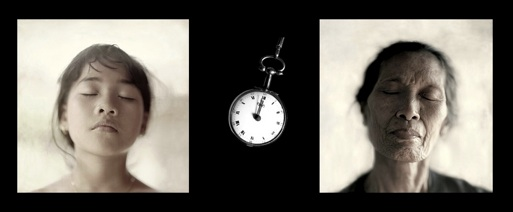
\includegraphics[width=.50\textwidth, keepaspectratio]{aging.jpg}
}
\fancyfoot[R]{

\includegraphics[height=.50in, keepaspectratio]{ucberkeley.jpg}

\includegraphics[height=.50in, keepaspectratio]{berkeleylab.jpg}
}
\fancyfoot[L]{
}
\renewcommand{\headrule}{}
\setlength{\voffset}{-0.25in}
\setlength{\headheight}{0.75in}
\setlength{\headwidth}{\textwidth}
}

\fancyfootoffset[L]{0.75in}
\fancyfootoffset[R]{0.75in}

\pagestyle{plain}

\begin{document}

\title{Bioinformatics Research Opportunity}
\date{\vspace{-0.75cm}Fall 2014}
\maketitle

\paragraph{} % Description

The Center for Research and Education on Aging (CREA) is a joint Lawrence
Berkeley National Laboratory and University of California, Berkeley institution.
Our mission is to investigate the basic processes that cause aging, with the
goal of improving and extending human life span.
We have been researching and developing software to automate the construction of biomedical knowledge bases,
with a focus on constructing a knowledge base that describes the human aging process.
We're seeking University of Waterloo students interested in doing volunteer research and  making open
contributions to the project. The goal is to further progress enough to give a presentation at
the International Conference on Bioinformatics later next year.

\paragraph{Expectations}

\begin{itemize}
\item Available to meet on Skype for about 30 minutes per week.
\item A volunteer time commitment of about 4-6 hours per week.
\end{itemize}

\paragraph{Requirements}

\begin{itemize}
\item Enrolled in an Undergraduate Program at the University of Waterloo.
\item Has completed at least one computing course, or has equivalent experience.

\end{itemize}

\paragraph{Desirable Experience}

\begin{itemize}
\item Breadth of knowledge in software development.
\item Good software implementation skills.
\newline
\item Prior experience in linguistics.
\item A formal understanding of English grammar and sentence structure.
\newline
\item Experience in introductory statistics.
\item Knowledge of artificial intelligence and machine learning.
\newline
\item Prior knowledge of biology and bioinformatics.
\item An awareness of current aging theories.

\end{itemize}

\paragraph{How to Apply}

\begin{itemize}

\item If interested, please contact Mark Farrell at the following email address: m4farrel@csclub.uwaterloo.ca.
\item Please include your résumé and a brief description of why you would like to participate
in this research opportunity.
\end{itemize}

Applications close October 1st, 2014.

\end{document}


